\documentclass{sig-alternate}
%\usepackage{hyperref}
%\usepackage[stable]{footmisc}
%\usepackage{epsfig}
%\usepackage{textcomp}
\usepackage{times}
%\usepackage{amssymb}
\usepackage{graphicx}
%\usepackage{url}
%\usepackage{listings}
%\usepackage{comment}

\newcommand{\ie}{i.e.} 
\newcommand{\eg}{e.g.} 
\newcommand{\et}{et al. }

\sloppy

\begin{document}

\title{Pattern Discovery in Energy Consumption}

\numberofauthors{3}
\author{
\alignauthor
Xiufeng Liu \\
\affaddr{University of Waterloo}\\
\email{xiufeng.liu@uwaterloo.ca}
\alignauthor 
Lukasz Golab \\
\affaddr{University of Waterloo}\\
\email{lgolab@uwaterloo.ca}
\alignauthor 
Ihab F. Ilyas \\
\affaddr{University of Waterloo}\\
\email{ilyas@uwaterloo.ca}
}
\maketitle

\begin{abstract}
Smart electricity meters are replacing conventional meters worldwide and have enabled a new application domain: smart meter data analytics.  In this paper, we introduce SMAS, our smart meter analytics system, which demonstrates the actionable insight that consumers and utilities can obtain from smart meter data.  We implemented SMAS inside a relational database management system using open source tools: PostgreSQL and the MADLib machine learning toolkit.  In the proposed demonstration, conference attendees will interact with SMAS as electricity providers and consumers, and will perform various analyses on two real data sets.

The concept of sustainability is more and more established as an integral component in modern economies. A
major threat to sustainability is the escalating demand for energy resulting in the depletion of natural resources and a concomitant threat to the global climate from the emissions produced. Although tourism and its sub-sectors, such as transport, accommodation, and attractions, constitute an increasingly important part of many economies, their contribution to energy use is not well researched. Particularly, in popular tourist destinations, such as New Zealand, tourism could be a significant contributor to energy consumption. As every tourist relies on the provision of accommodation, this is considered a core sub-sector within tourism. Previous case studies have indicated that accommodation is an energy-intense sector, however, comprehensive research on energy use patterns is missing. This paper contributes to the understanding of energy use within the accommodation sector by analysing the New Zealand scenario. The main objectives are the exploration of differences in energy consumption between electricity data and water data, and  accommodation categories, and the role of factors such as business size in this consumption. Based on this analysis benchmarks are established for each category for total annual energy use and energy intensities, such as energy use per visitor night. When aggregated the total energy use of the accommodation sector in New Zealand is also estimated. The results reveal that hotels are the largest (net and per capita) energy consumers in the accommodation sector, making up 67\% of the total 1.74 PJ consumed in 1999 in the accommodation sector. 
\end{abstract}

\section{Introduction}

As conventional power grids turn into smart power grids, traditional electricity meters are being replaced by smart meters.  The main operational advantage of smart metering systems is their ability to automatically collect fine-grained (typically hourly) electricity consumption data, which enables accurate billing without having to send workers to customer premises to manually read the meters.  Additionally, a new application area has emerged: smart meter data analytics.  The vast amounts of data collected by smart metering systems can help understand electricity consumption patterns, thereby helping governments and utilities plan for the future and helping consumers reduce their bills.  The market for smart grid data analytics is growing rapidly and is expected to reach over \$4 billion by the year 2020\footnote{http://www.greentechmedia.com/research/report/the-soft-grid-2013}.

Some database vendors currently offer smart meter analytics software, e.g., SAP\footnote{http://www.sap.com/pc/tech/in-memory-computing-hana/software/ smart-meter-analytics/index.html} and Oracle/Data Raker\footnote{http://www.oracle.com/us/products/applications/utilities/meterdata-analytics/index.html}.  There are also several startups in this area, e.g., C3Energy.com and OPower.com, and a recent research prototype system \cite{jarrah}.  However, these systems focus on simple aggregation and ways of visualizing electricity consumption.  On the other hand, a number of advanced smart meter mining techniques have been proposed, mostly in the smart grid and machine learning literature, but the focus has been on the insights that can be obtained from the data rather than algorithm and system implementation.  In this paper, we introduce our smart meter analytics system, SMAS, which is unique in at least two ways:

\begin{enumerate}

\item In addition to simple visualization and temporal aggregation, SMAS supports state-of-the-art smart meter data mining techniques, including those for extracting daily consumption profiles \cite{omid} and understanding the effect of temperature on consumption \cite{birt}.  The patterns and features identified by these algorithms can be used for clustering similar consumers (which is useful for designing targeted customer engagement programs), forecasting electricity consumption and providing personalized feedback to consumers.

\item Rather than using separate systems for data storage and analysis (as was done in \cite{jarrah}), we implemented SMAS entirely inside an open-source relational Database Management System.  Specifically, we used PostgreSQL and the MADLib in-database machine learning toolkit \cite{madlib}.

\end{enumerate}  

In Section~\ref{sec:system}, we describe the system architecture of SMAS and the supported algorithms and analytics.  In Section~\ref{sec:demo}, we outline the functionalities of SMAS that will be demonstrated, which will show the kinds of insights that can be obtained from real smart meter data sets.  Conference attendees will interact with SMAS in two ways.  As electricity consumers, they will see how their consumption ranks against that of their neighbours, and they will obtain advice on how to change their consumption habits to lower their bills and reduce their carbon footprint.  As electricity providers, they will be able to understand the different types of consumers and predict future consumption.

By demonstrating SMAS, we hope to increase the awareness of the emerging application area of smart meter analytics within the data management community.  We also hope to stimulate further research on this topic, especially on applying novel database technologies such as column-stores, in-database machine learning and distributed data processing to improve the efficiency and effectiveness of smart meter analytics.  We plan to make SMAS freely available online for others to use and extend. 

%\section{System Overview} \label{sec:system}
%Figure~\ref{fig:architecture} shows the architecture of SMAS.  The real-time layer consumes raw smart meter data and runs simple alerting queries, such as those which detect very high consumption readings.  The batch layer packages raw data into chunks that are batch-loaded into the analytics database, e.g., once an hour or once a day.  The batch layer also accepts bulk-uploads, e.g., historical consumption data from legacy systems.  The analytics layer, which is the focus of this paper, consists of an underlying database, analytics libraries, and a Web front-end.  In addition to the consumption time series generated by smart meters, the database also contains the location of each consumer and hourly temperature data obtained from a local weather station.  Thus far, we have implemented the analytics layer; we envision implementing the real-time layer using a data stream engine and the batch layer using a database system or Hadoop/Hive.

%Figure~\ref{fig:analyticslayer} shows the design of the analytics layer, which uses PostgreSQL as the database and MADLib as the (in-database) machine learning library.  Furthermore, we use Highcharts (www.highcharts.com) as the visualization engine, and Tomcat as the web application server.  The main functionalities of SMAS include consumer feedback, segmentation (clustering) analysis and forecasting.  Each of these tasks requires a set of features and patterns to be extracted from the data (which are then stored in materialized views).  We employ three algorithms for feature extraction, as detailed below. 
%The implemented analytics modules include load analysis, pattern discovery, segmentation, forecasting and feedback services. The future extensions may include using the PostgreSQL-XL cluster (www.postgres-xl.org) for  big data workload, applying columnar store to PostgreSQL (citusdata.github.io/cstore\_fdw), and the support for R, and Matlab. 
\section{Problem Statement}
A high-level schematic of the thermal
profiling methodology proposed here is given in Figure
1. We observe hourly-sampled energy consumption time
series (measured in kWh) {Xt}n and outside temperature
time series {Tt}n for premises (users) n = 1, ..., N. In the
Decoding step we would like to separate the signal {Xt} for
a given user n into time-consistent portions that are (linearly)
driven by temperature, and segments that are not affected by
temperature. In effect, we cluster the observations in {Xt}
according to how they change over time with changes in
{Tt}. To achieve this we allow the premise to experience
regimes, or occupancy states characterized by different
levels of activity over time. In addition, we explicitly model a
temperature-dependent probability of the premise performing
heating or cooling. This formulation is based on the following
observations: i) heating or cooling spells generally span
multiple hours, and given a certain response (say heating) at
a given hour, it is likely that the next hour will see the same
thermal activity; ii) while the premise may have appliances
that work on pre-determined schedules (e.g., an automatic
thermostat that maintains inside temperature within a certain
admissible range), these settings may change dynamically
based on user preferences and occupancy, and iii) heating or
cooling appliances do not consume fixed amounts of energy
when they are on, but undergo different operational regimes
depending on how much work is needed to respond to the
outside temperature experienced.

\section{The Data Sets}
We have the time series data of electricity and water. 

{\bf Electricity Data.}
This dataset is the electricity consumption data of 27,300 customers in Southwestern Ontario Canada collected between 2011 and 2012 at an hourly time resolution. There are 350,319,041 data points in total, roughly 10GB. The data set does not have any missing values. The weather temperature at the same period are from Envoronment Canada (www.ec.gc.ca), which are also time-series data at hourly interval. 

{\bf Water Data.}
This data set is the water consumption data of 25,858 customers in Abbotsford city, Britian Columnbia, Canada collected between September 1, 2012 and August 31, 2013 at an hourly time resolution. There are 215,172,496 data points in total, roughly 10GB. However, in this data set, we have more information about the types of the customers. The types of the customers and the proporation of the data points are as follows:  SFRES (78.6\%), agriculture (10.6\%), MFRES (4.71\%), commercial (2.49\%),  industry (1.94\%), institution (1.57\%), residential (0.025\%),  SFRES\_MUM (0.025\%), INSTITUTIONAL (0.0004\%). We make the qualitity check of the data, and remove the obvious outliers and errors. We also get corresponding hourly weather data  from Environment Canada, including weather temperature and condition (\ie, clear, rain, drizzle, snow, etc).

\section{Analytics Methods}
\subsection{Thermal Profiling}
An important factor that needs to be consider is the impact of weather on the consumption of electricity and water. The external temperature is correlative to the electricity consumption of customers. For example, in winter, the consumption rises with the decreasing of the  temperature due to the heating, while in summer, the consumption rises  due to the cooling.  %Birt \et  \cite{birt} use three piecewise linear regression lines to mode the relationship between temperature and the electricity use. The scatter plot in Figure~\ref{fig:threelmodel} illustrates the three linear lines model of a customer. Each point is the particular hourly consumption under the corresponding outdoor temperature. The algorithm computes two regression models: one corresponding to the 90th percentile consumption at each temperature and one corresponding to the 10th percentile at each temperature. As shown in Figure~\ref{fig:threelmodel}, the reveal several interesting features for each customer, including \emph{cooling gradient} which is the slope of the 90th percentile line corresponding to high temperature, the \emph{heating gradient} which is the slope of the line corresponding to low temperature, and  the \emph{base load} which is the height of the 10th percentile lines at their lowest point (corresponds to load due to appliances that are always on, such as a refrigerator). The customers with high heating gradient values might have air conditions at a low temperature setpoints or have used ineffcient cooling conditions.  
%\begin{figure}[t]
%\centering
%
\includegraphics[width=0.45\textwidth]{images/threelmodel}
%\caption{The piecewise linear regression model}
%\label{fig:threelmodel}
%\end{figure}
We will use the algorithm of peroidic auto-regression with the exogonous vaiables (PARX) \cite{omid}  to extract load regardless of the outdoor temperature, as illustrated in Figure~\ref{fig:dailyprofile}.  On the left, the figure shows a fragment of the hourly consumption time series for some consumer over a period of several days. We can only collect the total hourly consumption reported by the smart meter (the upper curve). The goal of the algorithm is to determine, for each hour, how much load is due to temperature (i.e., heating and cooling), and how much load is due to daily activity independent of temperature (the lower curve). Once this is determined, the algorithm fits a time series auto-regression model and computes the average temperature-independent consumption at each hour of the day, illustrated on the right of Figure~\ref{fig:dailyprofile} (the X-axis is the hour of the day and the Y-axis is the average consumption). Since weekday and weekend activities may differ, it is interesting to separately compute the typical weekday and weekend profiles for each consumer.
 
 \begin{figure}[t]
\centering
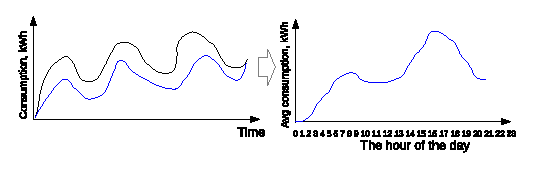
\includegraphics[width=0.5\textwidth]{images/dailyprofile}
\caption{Extracting daily consumption profiles}
\label{fig:dailyprofile}
\end{figure}

\subsection{Clustering}
{\bf Clustering on Shape.}
Our objective is to discover the representive daily load shapes of customers. 

{\bf K-Spectral Centroid Clustering.}

{\bf Clustering Goodness Estimation.}

\section{Results and Discussion}




\subsection{The Consumption Pattern of Electricity}

\subsubsection{The Pattern of Total Use}
We now describe how the features and patterns identified by the above algorithms enable the three functionalities of SMAS: consumption feedback, segmentation and forecasting. 

Feedback is important to consumers and is generated from the temperature regression models and daily profiles.  We use a rule-based feedback engine with a set of pre-specified rules that trigger different types of feedback as appropriate.  For instance, if we detect a high base load, we recommend replacing the refrigerator or another appliance that is always on, whereas a high value of the cooling gradient may indicate an inefficient air conditioning system.  Additionally, for jurisdictions with time-dependent electricity pricing such as the province of Ontario, if the daily profile shows high consumption during peak-pricing times, we recommend shifting some activities to off-peak times if possible.

Furthermore, SMAS can estimate a user's carbon footprint if the electricity generation sources and their carbon footprints are known (which they are in Ontario).  Given the carbon cost of consuming a kilowatt-hour of electricity at various times of the day, and assuming that all the consumers are provided electricity from exactly the same set of sources, it is straightforward to compute the carbon footprint of an individual consumer.  Usually, the carbon cost of electricity production increases during peak demand times, when additional power plants, which are often dirty coal power plants, must be used.  Thus, SMAS can generate feedback for reducing the carbon footprint if a given consumer's peak demand coincides with a high carbon cost. 

Segmentation and forecasting are important to utilities.  SMAS supports K-means clustering based on the features we discussed earlier, namely base load, heating and cooling gradients and the daily profiles.  For example, clustering on daily profiles can reveal groups of consumers with similar lifestyles, and the utility may design targeted energy-saving programs for each group.  Moreover, SMAS can use the temperature dependence and daily profile, along with a temperature forecast, to predict future demand.  Additionally, we implemented several time series forecasting algorithms, including ARIMA and Holt-Winters.
%SMAS has integrated the forecast algorithms, including PARX, ARIMA, and exponential smoothing HoltWinters (the screenshot is not shown due to space reason). 

In future work, we plan to add more algorithms and analytics to SMAS.  However, we believe that the algorithms and analytics we currently support are a representative set and can illustrate the kinds of insights that can be obtained from smart meter data.

\subsubsection{The Pattern of Activity Consumption}

\subsection{The Consumption Pattern of Water}

\section{Related Work}


\section{Conclusion and Future Work} 


%\raggedright
%\flushleft
\begin{thebibliography}{20}

\bibitem{omid}
O.~Ardakanian, N.~Koochakzadeh, R.~P.~Singh, L.~Golab, and S.Keshav, Computing Electricity Consumption Profiles from Household Smart Meter Data, in Proc. of the EDBT Workshop on Energy Data Management (EnDM), 140-147, 2014.

\bibitem{birt}
B.~J.~Birt,  G.~R.~Newsham,  I.~Beausoleil-Morrison, M.~M.~Armstrong,  N.~Saldanha, and I.~H.~Rowlands, Disaggregating Categories of Electrical Energy End-use from Whole-house Hourly Data, Energy and Buildings, 50:93-102, 2012.

\bibitem{madlib}
 J.~M.~Hellerstein, C.~R\'{e}, F.~Schoppmann, D.~Wang, E.~Fratkin, A.~Gorajek, and A.~Kumar. The MADlib Analytics Library: or MAD Skills, the SQL. PVLDB, 5(12):1700--1711, 2012.

\bibitem{jarrah}
A.~J. Nezhad, T.~K.~Wijaya, M.~Vasirani, and K.~Aberer.  SmartD: Smart Meter Data Analytics Dashboard, in Proc. Int. Conf. on Future Energy Systems (ACM e-Energy), 213-214, 2014.

%\bibitem{benchmarking}
%X.~Liu, L.~Golab,  and I.~Ilyas. Benchmarking of Smart Meter Data Analytics. In Submission, 2014.

\end{thebibliography}

%\appendix
\end{document}
